\label{wordHistogram}
Write a function that counts occurrences of each word in a string and
returns a list. The counts must be organized as a list of trees using the
following \lstinline{Tree} type:
\begin{quote}
  \mbox{\lstinline! type Tree = Node of char * int * Tree list!}
\end{quote}
An illustration of a value of this type is shown in Figure~\ref{fig:treeType}
\begin{figure}
  \centering
  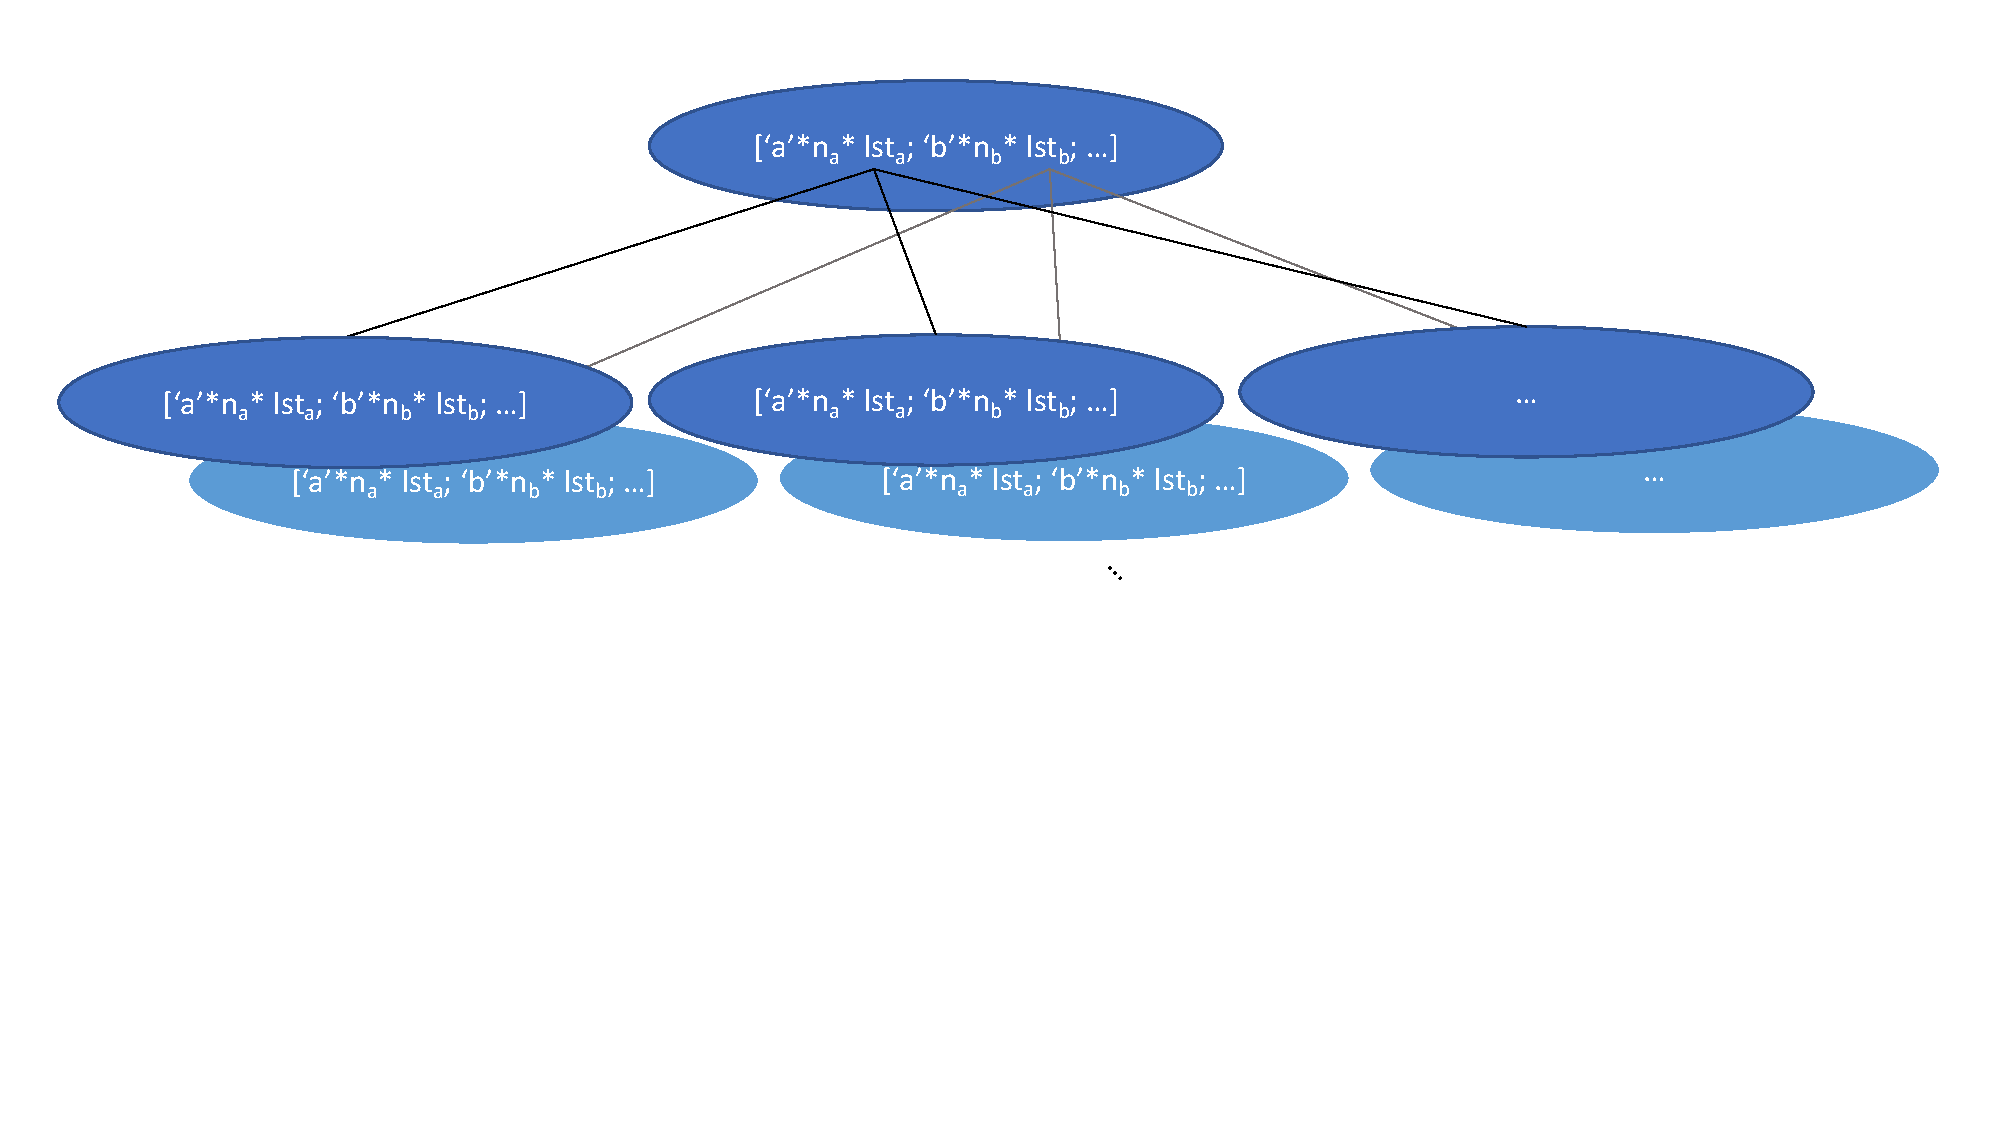
\includegraphics[width=\textwidth]{treeType}
  \caption{An illustration of a list of values of the type \lstinline{Tree}.}
  \label{fig:treeType}
\end{figure}
Words are to be represented as the sequence of characters from the
root til a node. The associated integer to each node counts the
orrucurence of a word ending in that node. Thus, if the count is 0, then
no words with that end point has occurred. For example, a string with the
words ``a abc ba'' should result in the following tree,
\begin{quote}
  \mbox{\lstinline![Node ('a', 1, [Node ('b', 0, [Node ('c', 1, [])])]);!}\\
  \mbox{\hspace{0.5em}\lstinline!Node ('b', 0, [Node ('a', 1, [])])]!}
\end{quote}
Notice, the counts are zero for the combinations ``ab'' and ``b'',
which are words not observed in the string. The function must have the type:
\begin{quote}
  \mbox{\lstinline!wordHistogram : src:string -> Tree list!}
\end{quote}
Write a program which reads the text \lstinline[language=console]{littleClausAndBigClaus.txt}, discard all characters that are not in \lstinline{['a'..'z', 'A'..'Z',' ']}, convert all the remaining characters to lower case, and calculate the occurence of the remaining words as a \lstinline{Tree list} type.
